\documentclass[pdf]{beamer}
%\mode<presentation>{}

\usepackage{amssymb,amsmath,amsthm,enumerate,mathtools}
\usepackage[utf8]{inputenc}
\usepackage{array}
\newcolumntype{C}[1]{>{\centering\arraybackslash}m{#1}}

\usepackage{verbatim}
\usepackage[parfill]{parskip}
\usepackage{graphicx}
\usepackage{caption}
\captionsetup[figure]{labelformat=empty}
\usepackage{subcaption}
\usepackage{bm}
\usepackage{amsfonts,amscd}
%\usepackage{gensymb}
\usepackage[]{units}
\usepackage{listings}
\usepackage{multicol}
\usepackage{tcolorbox}
\usepackage{physics}
\usepackage{multirow}
\usepackage{pgfplots}
\pgfplotsset{compat=1.7}
\usepackage{hyperref}
\hypersetup{
    colorlinks=true,
    linkcolor=franklinblue,
    filecolor=magenta,      
    urlcolor=cyan,
    bookmarks=true,
    citecolor= black
    % pdftitle={Overleaf Example},
    % pdfpagemode=FullScreen,
    }
\usepackage{colortbl}
\usepackage{booktabs}
\usepackage{gensymb}
\usepackage{color}
\usepackage{natbib}

\usepackage{tikz}
\usepackage{fixltx2e}
\usepackage[english]{babel}
\usepackage[absolute,overlay]{textpos}
%\usepackage{gnuplottex} % For t-distribution using gnuplot.
%The following function is use in students t distribution. 
% \def\btextttasefunc{    gamma((\n+1)/2.)/(sqrt(\n*pi)*gamma(\n/2.))*((1+(x*x)/\n)^(-(\n+1)/2.))}    
% \def\n{7}
%\usepackage{tkz-fct} % For t-distribution plotting.
% \usepackage{pst-func} % For t-distribution plotting.
\usepackage{longtable}
\usepackage{changepage} 

\usetikzlibrary{shapes,decorations,arrows,calc,arrows.meta,fit,positioning}
\tikzset{
    -Latex,auto,node distance =1 cm and 1 cm,semithick,
    state/.style ={ellipse, draw, minimum width = 0.7 cm},
    point/.style = {circle, draw, inner sep=0.04cm,fill,node contents={}},
    bidirected/.style={Latex-Latex,dashed},
    el/.style = {inner sep=2pt, align=left, sloped}
}

%Normal Distribution
\pgfmathdeclarefunction{gauss_}{2}{\pgfmathparse{1/(#2*sqrt(2*pi))*exp(-((x-#1)^2)/(2*#2^2))}%
}
%Gamma Distribution
\pgfmathdeclarefunction{gammaPDF}{2}{
\pgfmathparse{1/(#2^#1*gamma(#1))*x^(#1-1)*exp(-x/#2)}
}

%%%%% For https://tikz.net/gaussians/ %%%%%

\usepackage{amsmath} % for \dfrac
\usepackage{tikz}
\tikzset{>=latex} % for LaTeX arrow head
\usepackage{pgfplots} % for the axis environment
\usepackage{xcolor}
\usepackage[outline]{contour} % halo around text
\contourlength{1.2pt}
\usetikzlibrary{positioning,calc}
\usetikzlibrary{backgrounds}% required for 'inner frame sep'
%\usepackage{adjustbox} % add whitespace (trim)

% define gaussian pdf and cdf
\pgfmathdeclarefunction{gauss}{3}{%
  \pgfmathparse{1/(#3*sqrt(2*pi))*exp(-((#1-#2)^2)/(2*#3^2))}%
}
\pgfmathdeclarefunction{cdf}{3}{%
  \pgfmathparse{1/(1+exp(-0.07056*((#1-#2)/#3)^3 - 1.5976*(#1-#2)/#3))}%
}
\pgfmathdeclarefunction{fq}{3}{%
  \pgfmathparse{1/(sqrt(2*pi*#1))*exp(-(sqrt(#1)-#2/#3)^2/2)}%
}
\pgfmathdeclarefunction{fq0}{1}{%
  \pgfmathparse{1/(sqrt(2*pi*#1))*exp(-#1/2))}%
}

\colorlet{mydarkblue}{blue!30!black}

% to fill an area under function
\usepgfplotslibrary{fillbetween}
\usetikzlibrary{patterns}
\pgfplotsset{compat=1.12} % TikZ coordinates <-> axes coordinates
% https://tex.stackexchange.com/questions/240642/add-vertical-line-of-equation-x-2-and-shade-a-region-in-graph-by-pgfplots

% plot aspect ratio
%\def\axisdefaultwidth{8cm}
%\def\axisdefaultheight{6cm}

% number of sample points
\def\N{50}

%%%%% End for https://tikz.net/gaussians/ %%%%%

\setbeamertemplate{caption}[numbered]

%new commands
\newcommand{\der}[2]{\frac{d#1}{d#2}}
\newcommand{\nder}[3]{\frac{d^#1 #2}{d #3 ^ #1}}
\newcommand{\pder}[2]{\frac{\partial #1}{\partial #2}}
\newcommand{\npder}[3]{\frac{\partial ^#1 #2}{\partial #3^#1}}
\newcommand{\sentencelist}{def}
\newcommand{\overbar}[1]{\mkern 1.5mu\overline{\mkern-1.5mu#1\mkern-1.5mu}\mkern 1.5mu}
\newcommand{\lined}{\overbar}
\newcommand{\perm}[2]{{}^{#1}\!P_{#2}}
\newcommand{\comb}[2]{{}^{#1}C_{#2}}
\newcommand{\intall}{\int_{-\infty}^{\infty}}
\newcommand{\Var}[1]{\text{Var}\left(#1\right)}
\newcommand{\E}[1]{\text{E}\left(#1\right)}
\newcommand{\define}{\equiv}
\newcommand{\diff}[1]{\mathrm{d}#1}
\newcommand{\empy}[1]{{\color{cadetblue}\texttt{#1}}}
\newcommand{\empr}[1]{{\color{franklinblue}\textbf{#1}}}
%https://tex.stackexchange.com/questions/192358/quickly-changing-all-the-file-paths-in-a-tex-file
%\newcommand{\pathtopdf}{C:/Users/bkwei/OneDrive - Franklin University/Desktop/Math_215/Data/IMDB/Processed} - Not Tested!
\newcolumntype{L}[1]{>{\raggedright\let\newline\\\arraybackslash\hspace{0pt}}m{#1}}
\newcolumntype{C}[1]{>{\centering\let\newline\\\arraybackslash\hspace{0pt}}m{#1}}
\newcolumntype{R}[1]{>{\raggedleft\let\newline\\\arraybackslash\hspace{0pt}}m{#1}}

\theoremstyle{remark}
\newtheorem*{remark}{Remark}
\theoremstyle{definition}

\newcommand{\examplebox}[2]{
\begin{tcolorbox}[colframe=darkcardinal,colback=boxgray,title=#1]
\end{tcolorbox}}

\newcommand{\eld}[1]{\frac{d}{dt}(\frac{\partial L}{\partial \dot #1}) - \frac{\partial L}{\partial #1}=0}
\newcommand{\euler}[1]{\frac{\partial L}{\partial #1}-\frac{d}{dt}(\frac{\partial L}{\partial \dot #1})}
\newcommand{\eulerg}[1]{\frac{\partial g}{\partial #1}-\frac{d}{dt}(\frac{\partial g}{\partial \dot #1})}
\newcommand{\divg}[1]{\nabla\cdot #1}
\newcommand{\prob}[1]{P(#1\vert I)}

\AtBeginSection[]{
  \begin{frame}
  \vfill
  \centering
  \begin{beamercolorbox}[sep=8pt,center,%shadow=true,
  rounded=true]{section}
    \LARGE
    \usebeamerfont{section}
    %\usebeamercolor[fg]{section}\inserttitle %\insertsectionhead\par%
    \setbeamercolor{section}{fg=white,bg=white}\insertsectionhead\par%
  \end{beamercolorbox}
  \vfill
  \end{frame}
}

\usetheme{Franklin} 
\def \i  {\item}
\def \ai {\item[] \quad \arrowbullet}
\newcommand \si[1]{\item[] \quad \bulletcolor{#1}}
\def \wi {\item[] \quad $\ \phantom{\Rightarrow}\ $}
\def \bi {\begin{itemize}\item}
\def \ei {\end{itemize}}
\def \be {\begin{equation*}}
\def \ee {\end{equation*}}
\def \bie {$\displaystyle{}
\def \eie {{\ }$}}
\def \bsie {\small$\displaystyle{}
\def \esie {{\ }$}\normalsize\selectfont}
\def \bse {\small\begin{equation*}}
\def \ese {\end{equation*}\normalsize}
\def \bfe {\footnotesize\begin{equation*}}
\def \efe {\end{equation*}\normalsize}
\renewcommand \le[1] {\\ \medskip \lefteqn{\hspace{1cm}#1} \medskip}
\def \bex {\begin{example}}
\def \eex {\end{example}}
\def \bfig {\begin{figure}}
\def \efig {\end{figure}}
\def \btheo {\begin{theorem}}
\def \etheo {\end{theorem}}
\def \bc {\begin{columns}}
\def \ec {\end{columns}}
\def \btab {\begin{tabbing}}
\def \etab {\end{tabbing}\svneg\svneg}
\newcommand \col[1]{\column{#1\linewidth}}
\def\vneg  {\vspace{-5mm}}
\def\lvneg {\vspace{-10mm}}
\def\svneg {\vspace{-2mm}}
\def\tvneg {\vspace{-1mm}}
\def\vpos  {\vspace{5mm}}
\def\lvpos {\vspace{10mm}}
\def\svpos {\vspace{2mm}}
\def\tvpos {\vspace{1mm}}
\def\hneg  {\hspace{-5mm}}
\def\lhneg {\hspace{-10mm}}
\def\shneg {\hspace{-2mm}}
\def\thneg {\hspace{-1mm}}
\def\hpos  {\hspace{5mm}}
\def\lhpos {\hspace{10mm}}
\def\shpos {\hspace{2mm}}

\logo{
\includegraphics[height=0.4in]{./style_files_franklin/FranklinUniversity_TM1.jpg}}

\title{BUSA 603}
\subtitle{Module 4:   Introducing A/B Testing, Experimental Designs, \\ and Analyzing Test Results}

\beamertemplatenavigationsymbolsempty

\begin{document}

\author[B. Weikel, Franklin University]{
	\begin{tabular}{c} 
	\Large
	Brian Weikel\\
    \footnotesize \href{mailto:brian.weikel@franklin.edu}{brian.weikel@franklin.edu}
    \vspace{1ex}
\end{tabular}
\vspace{-4ex}}

\institute{
	
\includegraphics[height=0.4in]{./style_files_franklin/FranklinUniversity_TM1.jpg}\\
	Business Analytics\\
	Franklin University}

\date{Spring 2024}%{\today}

\begin{noheadline}
\begin{frame}[t]\maketitle\end{frame}
\end{noheadline}

\begin{frame}[t]{Outline\footnote{These lecture notes map to chapters 8, 9 and 13 of \cite{davis2022}.}}
\begin{enumerate}
\item  A/B Testing
\vspace{1.5ex}
\item Experimental Design
\vspace{1.5ex}
\item Basic Principles of Statistical Testing
\vspace{1.5ex}
\item Analyzing Results
\vspace{1.5ex}
\item Appendix
\end{enumerate}
\end{frame}

\section{A/B Testing}

\begin{frame}[t]{A/B Testing}
\empr{A/B testing} is a method for testing the effectiveness of a marketing effort, such as an advertising campaign, via a controlled experiment that tests two or more conditions before exposure to the broader marketplace. \\
\vspace{0.5ex}
\small
\begin{itemize}
\item A/B testing is based on the Scientific Method, a principle used in many ways across many science fields.
\item A/B testing is also sometimes called \empr{split testing} or \empr{bucket testing} because audiences members are split, or audience members are placed in different buckets, to see response to different marketing inputs. These terms are generally used synonymously.
\item A/B testing is also sometimes called \empr{A/B/N testing}, signifying that more than two inputs can be tested at the same time (N is used to signify any number). 
\end{itemize}
\end{frame}

\begin{frame}[t]{Scientific Method}
\begin{figure}[htbp]
  \captionsetup{justification=centering}
  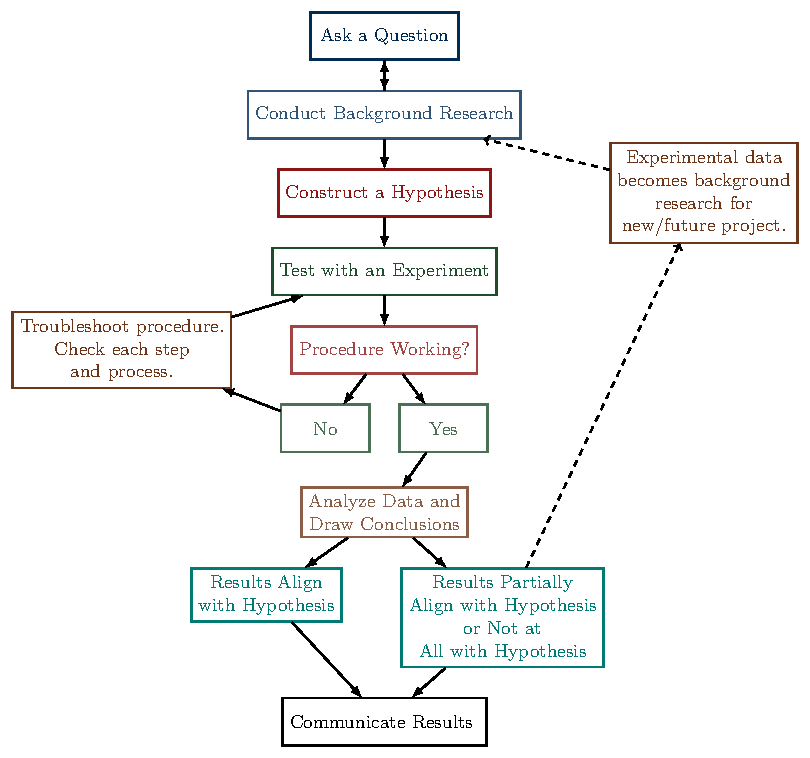
\includegraphics[height=7.1cm, trim=1.0cm 0.3cm 1.0cm 0.6cm width=7.1cm]{Scientific_Method.pdf}
  \caption{Figure {\color{franklinblue} 1}: The Scientific Method}
\end{figure}
\end{frame}

\begin{frame}[t]{Conducting an A/B Test is Quantitative Research}
\empr{Quantitative research} involves structured data collection methods that provide results that can be converted to numbers and analyzed through statistical procedures. Statistical testing, such as A/B testing, is a quantitative research method.\\
\vspace{1.5ex}
\empr{Qualitative research} involves unstructured data collection methods where results are subjectively interpreted.\\
\vspace{0.5ex} 
\small
\begin{itemize}
\item Qualitative research is typically used for initial exploratory research.  However, it can also be used after a descriptive study to explore deeper into the minds of consumers or whoever the research participants may be. 
\item Since qualitative research involves probing via open-ended questions, the results become
subjective. That makes generalizing the findings to a larger population or other consumers more
difficult.  
\item The textbook refers to qualitative research approaches as \textit{intuitive}.
\end{itemize}
\end{frame}

\begin{frame}[t]{Benefits and Costs of Different Research Approaches}
\small
\begin{table}[htbp]
  \centering
  \captionsetup{justification=centering}
    \begin{tabular}{|ccc|}
    \toprule
   \textbf{{\color{franklinblue} Feature }} & \textbf{{\color{franklinblue} Qualitative\footnote{For a deeper understanding of qualitative research approaches see \cite{calder1977}.}}} & \textbf{{\color{franklinblue} Quantitative}}  \\
    \midrule
                           & Exploratory, & Descriptive, \\
    \textbf{Research Type} & Clinical, & Scientific, \\
                           & Phenomenological & Causal\\
    \midrule
    \textbf{Sample Size} & Small & Large \\
    \midrule
    \textbf{Question Types} & Unstructured & Structured \\    
    \midrule
    \textbf{Type of Analysis} & Subjective & Objective, statistical \\
    \midrule
    \textbf{Generalizability} & Limited & High \\
    \midrule
    \textbf{Costs} (Typically) & Lower & More expensive \\
    \midrule
    \textbf{Time Frame} (Typically) & Shorter & Longer \\
  \bottomrule
     \end{tabular}%
  \caption{Comparison of Qualitative and Quantitative Research}
  \label{tab:cqqr}%
\end{table}%
\end{frame}


\begin{frame}[t]{A Few Marketing Research Approaches}
\scriptsize
\begin{table}[htbp]
  \centering
  \captionsetup{justification=centering}
    \begin{tabular}{|cccc|}
    \toprule
   \multirow{2}*{\textbf{{\color{franklinblue} Method }}} & \multirow{2}*{\textbf{{\color{franklinblue} Approach}}} & \textbf{{\color{franklinblue} Knowledge}} & \multirow{2}*{\textbf{{\color{franklinblue} Rationale}}} \\
   & & \textbf{{\color{franklinblue} Type}} & \\ 
    \midrule
     \multirow{11}*{Quantitative} & \multirow{4}*{Descriptive} &  \multirow{4}*{Everyday} & To find numerical patterns \\
     & & &  related to everyday concepts.  \\
      & & & As an example, consumption  \\
      & & & breakdowns by age.\footnote{In the field of data science, this is called exploratory data analysis, or EDA.  A classic reference is \cite{tukey1977}.  A rather recent survey of EDA tools is \cite{ghosh2018}.} \\
    \cmidrule{2-4}
    &  \multirow{3}*{Scientific} &  \multirow{3}*{Scientific} &  To use numerical measurement \\
    & & & to test scientific theories and\\
    & & &  constructs. \\  
    \cmidrule{2-4}
    &  \multirow{4}*{Causal} &  \multirow{4}*{Causal} &  To use numerical measurement \\
    & & & to test causal hypotheses using\\
    & & & data from randomized control trials \\
    & & & or observational data studies. \\
  \bottomrule
     \end{tabular}%
  %\caption{Summary of a Few Research Approaches}
  %\label{tab:sra}%
\end{table}%
\end{frame}

\begin{frame}[t]{A Few Marketing Research Approaches Continued}
\scriptsize
\begin{table}[htbp]
  \centering
  \captionsetup{justification=centering}
    \begin{tabular}{|cccc|}
    \toprule
   \multirow{2}*{\textbf{{\color{franklinblue} Method }}} & \multirow{2}*{\textbf{{\color{franklinblue} Approach}}} & \textbf{{\color{franklinblue} Knowledge}} & \multirow{2}*{\textbf{{\color{franklinblue} Rationale}}} \\
   & & \textbf{{\color{franklinblue} Type}} & \\ 
    \midrule
     \multirow{12}*{Qualitative}& \multirow{4}*{Exploratory} & \multirow{4}*{Prescientific} &  To generate scientific \\
     & & & constructs and to  \\
     & & & validate them against \\
     & & & everyday experience.\\
    \cmidrule{2-4}
    & \multirow{5}*{Clinical} & \multirow{5}*{Quasi-scientific} &  To use second-degree \\
    & & & scientific constructs \\
    & & & without numerical  \\ 
    & & & measurement. For example, \\
    & & & the use and examination \\    
    & & & of clinical judgments. \\  
    \cmidrule{2-4}
     & \multirow{2}*{Phenomenological} & \multirow{2}*{Everyday} &  To understand the everyday \\ 
    & & & experience of the consumer.\\
  \bottomrule
     \end{tabular}%
  \caption{Summary of a Research Approaches}
  \label{tab:sra}%
\end{table}%
\end{frame}

\begin{frame}[t]{A/B Testing Stages}
The goal of A/B testing in marketing is to identify differences in marketing outcomes after the random assignment of people to marketing input A or marketing input B. \\
\vspace{1.5ex}
It is called A/B testing because oftentimes two conditions are tested and these conditions are called condition A and condition B. \\
\vspace{1.5ex}
A/B testing occurs in two stages. \\
\vspace{1.5ex}
\begin{itemize} 
  \item \empr{Exploration stage}
  \item \empr{Exploitation stage} 
\end{itemize}
\end{frame}

\begin{frame}[t]{Exploration Stage}
In the exploration stage, the marketing analytics professional chooses what portion of the potential audience to explore. \\
\vspace{1.5ex} 
Then A/B testing software randomly selects people to assign to the exploration stage. \\
\vspace{1.5ex}
The software then again uses randomization to assign a proportion of those chosen for the exploration stage to be exposed only to version A, and one less that proportion to version B.\footnote{At times you may hear one version called ``test'' and the other version called ``control'', where ``test'' refers to a new treatment, method, structure, \ldots and ``control'' is the existing treatment, method, structure, \ldots }  \\
\vspace{0.5ex}
\small
\begin{itemize}
\item The proportion is usually, but not always, a half.  
\item Those who see version A never know a version B exists, and vice versa.
\item Assigning people to see different conditions is now much easier in the digital world than it is in the physical world.
\end{itemize}
\end{frame}

\begin{frame}[t]{Exploitation Stage}
Upon completion of the exploration stage, software determines which version was more successful. \\
\vspace{1.5ex} 
The marketing analytics professional tells the software algorithm what marketing outcome is important in order to test whether version A or B is more successful (e.g., click-through rates, site duration, purchase conversion \ldots ). \\
\vspace{1.5ex}
\begin{itemize}
\item The winning version is exposed to the large remainder of the potential audience that was not part of the exploration stage. 
\item This exposure frequently happens automatically, but it is possible to set it up so that the marketing analytics professional is required to complete several steps before enacting the winning version.
\end{itemize}
\end{frame}

\begin{frame}[t]{New Approaches for A/B Testing}
\begin{enumerate}
\item \empr{Bandit testing} is very similar to A/B testing but differs in the exploitation stage.  
\begin{itemize}
\item As with A/B testing, bandit test's exploration stage compares multiple options such as versions A and B. 
\item Unlike A/B testing, bandit testing has an \underline{adaptive exploitation} \underline{stage}. Specifically, the software determines which version was more successful and exposes both versions to some of the remaining audience, proportionate to version successfulness.\footnote{In the exploitation stage of A/B testing, the successful campaign would go to all of the remaining people on the list, but bandit testing would send both the successful and unsuccessful campaigns to another smaller portion in a series of exploration stages, increasingly using the more successful campaign.}
\end{itemize}
\item Many software systems allow marketers to analyze the success of options during the exploration stage of A/B testing \underline{across} \underline{different segments} by applying the results intelligently across segments in the exploitation stage.
\end{enumerate}
\end{frame}

\begin{frame}[t]{Potential Challenges with A/B Testing}
Potential challenges with A/B testing include:\\
\vspace{1.5ex}
\small
\begin{enumerate}
\item One of the largest challenges with A/B testing is making decisions from a small sample of customers in the exploration stage or stopping an A/B test before a sufficient number has been tested.  To address this challenge, we will rely on statistical \empr{power}.  We introduce statistical power in a later section. 
\item  A \empr{false positive occurs} when a condition seems to be the winner in the exploration stage, but it does not actually perform as well in the exploitation stage. The chances of a false positive are much larger when too many dimensions are tested at once, especially without ample sample size.  We expand on false positives in a later section.
\end{enumerate}
\end{frame}

\begin{frame}[t]{Potential Challenges with A/B Testing Continued}
\small
\begin{enumerate}
  \setcounter{enumi}{2}
\item Running multiple tests at the same time with the same audience can create overlap and problem interactions. This happens when a version in one A/B test affects the perceptions of a version in another A/B test.
\item Distinguishing statistical significance from business significance. 
\item In order to rule out seasonality, A/B tests should be conducted for lengthy periods.
\item Hypotheses need to be be rigorously defined and vetted. 
\item While an A/B test may optimize a marketing mix variable with its current design, it may be a \empr{local maximum}. That is, there may exist designs that would yield a \empr{global maximum}.\footnote{For a more thorough review of A/B testing in the ad tech space, see \cite{kohavi2009},  \cite{kohavi2011}, and \cite{kohavi2017}.} 
\end{enumerate}
\end{frame}

\begin{frame}[t]{Tools for Running A/B Tests}
There are many online tools available for A/B testing.  The textbook recommends the following, which are not listed in any particular order. \\
\vspace{1.5ex}
\begin{columns}[T]
\begin{column}{0.5\textwidth}
\begin{enumerate}
\item \href{https://www.optimizely.com/}{Optimizely}
\vspace{1.0ex}
\item \href{https://vwo.com/}{VWO}
\vspace{1.0ex}
\item \href{https://www.convert.com/}{Convert Experiences}
\vspace{1.0ex}
\item \href{https://www.sitespect.com/}{SiteSpect}
\vspace{1.0ex}
\end{enumerate}
\end{column}
\begin{column}{0.5\textwidth}  %%<--- here
\begin{enumerate}
  \setcounter{enumi}{4}
\item \href{https://www.abtasty.com/}{AB Tasty}
\vspace{1.0ex}
\item \href{https://firebase.google.com/docs/ab-testing?sjid=15712676071402063705-NA}{Firebase A/B Testing}
\vspace{1.0ex}
\item \href{https://www.qubit.com/}{Qubit} 

\vspace{1.0ex}\item \href{https://business.adobe.com/products/target/adobe-target.html}{Adobe Target}
\vspace{1.0ex}
\end{enumerate} 
\end{column}
\end{columns}
See the textbook for a  few other marketing tools with A/B testing and crowdsourcing capabilities.\footnote{\empr{Crowdsourcing} is the practice of gathering information by requesting the services of a large number of people, typically through online connection. In general, crowdsourcing is not recommended for rigorous statistical testing since many potential biases may occur, such as \empr{voluntary response bias}, \empr{self-interest bias}, and \empr{social-desirability bias}, to name few.}
\end{frame}

\section{Experimental Design}

\begin{frame}[t]{Experiments}
It is wise to take time and effort to organize an experiment properly to ensure that the right type of data, and enough of it, is available to answer the questions of interest as clearly and efficiently as possible. This process is called \empr{experimental design}.\footnote{The National Institute of Standards and Technology 
%of the U.S. Department of Commerce
 has an informative introductory exposition on \href{https://www.itl.nist.gov/div898/handbook/pri/pri.htm}{experimental designs}.}
%http://www.stat.yale.edu/Courses/1997-98/101/expdes.htm
\begin{enumerate}
\item An \empr{experiment} deliberately imposes a treatment (or condition) on a group of objects or subjects in the interest of observing the response. \\
\vspace{1.5ex}
\begin{itemize}
\item An \empr{observational data study} involves collecting and analyzing data without changing existing conditions.\footnote{Three types of bias can arise in observational data: (i) confounding bias, (ii) selection bias (i.e, improper selection of participants through stratifying, adjusting or selecting), and (iii) measurement bias (i.e., imprecise or biased measurement of variables in analysis).} 
\end{itemize}
\end{enumerate}
\end{frame}

\begin{frame}[t]{Treatments and Factors}
\begin{enumerate}
  \item []
\begin{itemize}
\item  Because the validity of an experiment is directly affected by its construction and execution, attention to experimental design is extremely important.
\end{itemize}
\vspace{-0.5ex}
  \setcounter{enumi}{1}
\item In experiments, a \empr{treatment} is something that researchers administer to experimental units.  For example, a customer arriving on a landing page layout could be ``treated" (i.e., served) one of three different pages. 
\item A \empr{factor} of an experiment is a \underline{controlled independent} \underline{variable}; a variable whose \empr{levels} are set by the experimenter.  A factor is a general type or category of treatments.  
\begin{itemize}
\item Different treatments constitute different levels of a factor.
\item Example: Using a website's source of origin for a user, 3 different group's users are subjected to distinct landing pages.  The users are the units.  There is 1 factor, 'landing page type.'  The factor's levels are the 3 different landing pages.
\end{itemize}
\end{enumerate}
\end{frame}

\begin{frame}[t]{Experimental Bias}
Suppose a website designer wishes to evaluate a new site design.  Based on the availability of multiple web servers and after unit, integration, regression, and end-user acceptance testing, she persuades the firm's technology organization to conduct an experiment by using the new design between 12:01 AM and 12:00 PM, while using the existing design between 12:01 PM and 12:00 AM. \\
\vspace{1.5ex}
The {\color{red} problem} with this experiment is that the designer has neglected to \underline{control} the differences in customers.  For example, the marketing department knows that those who arrive between 12:01 PM and 12:00 AM tend to have a larger rate of employment, larger disposable income, and larger conversion rates. This is an example of \empr{experimental bias}. 
\end{frame}

\begin{frame}[t]{A Benefit of Randomization}
Because it is generally extremely difficult for experimenters to eliminate bias using only their expert judgment, the use of \empr{randomization} in experiments is common practice. 
\begin{itemize}
\item In a randomized experimental design, objects or individuals are randomly assigned to an experimental group. 
\item Using randomization is the most reliable method of creating \underline{homogeneous treatment groups}, without involving any potential biases or judgments. 
\item One caveat is that randomization is not perfect. By chance, it is possible that one group happens to have younger people on average than the comparison group.
\end{itemize}
\end{frame}

\begin{frame}[t]{Causal Inference}
Cause-and-effect approaches are extremely important because decision-makers are usually interested in knowing whether a marketing action might cause a desired marketing outcome, not just whether they happen to occur at the same time. More succinctly, they are interested in causation and not just correlation. \\
\vspace{1.5ex}
\empr{Causal inference} is the formal name for cause-and-effect interpretations of research methods like experiments.
\small
\begin{itemize}
\item \cite{rubin1974} and \cite{holland1986} are seminal papers in the modern development of causal inference in the statistical literature. 
\item An excellent introduction to causal inference from an econometric perspective is \cite{angrist2009}. 
\item On the use of Bayesian Networks to explain causality, see \cite{pearl2009} and \cite{pearl2018}. 
\end{itemize}
\end{frame}

\begin{frame}[t]{Requirements for Causal Inference}
Let $X$ be a factor, such as a marketing input. Let $Y$ be the outcome, such as a purchase conversion. For $X$ to cause $Y$: \\
\vspace{1.5ex}
\begin{enumerate}
\item $X$ must occur before $Y$ chronologically.
\item There must be evidence that $X$ is associated with $Y$.
\item Other causal factors are ruled out (e.g., “controlled for”).
\end{enumerate}
The assumption that other potential causal factors have been eliminated is almost always the most challenging of the three to realize. 
\end{frame}

\begin{frame}[t]{Sleeping with Shoes On}
It is important to emphasize that \underline{correlation is {\color{red} not} the same as} \underline{causation}. In general when two variables are correlated, we cannot conclude that changing the value of one variable will cause a change in the value of the other.\\
\vspace{1.5ex}
Consider the following example:\\
\small
\vspace{-0.0ex}
\begin{itemize}
\item Sleeping with one's shoes on is strongly correlated with waking with a headache. 
\item Sleeping with one's shoes on must cause headaches. 
\item Thus one should take off one's shoes before sleeping.
\end{itemize}
\normalsize
\vspace{-1.0ex}
 There is an error in the causal conclusion. What is a likely better explanation of the correlation?  
\end{frame}

\begin{frame}[t]{Sleeping with Shoes On Continued}
\underline{Solution}: There is a 3rd factor that is related to sleeping with one's shoes on and waking with a headache. Sleeping with one's shoes on is not as comfortable as sleeping sans shoes.  Thus one must not have all of his/her cognitive abilities prior to falling asleep.  For example, being inebriated. Intoxication is a \empr{confounder}. \\
\vspace{1.5ex}
A confounder is a variable that is related to both the treatment and the outcome. When a confounder is present, it is difficult to determine whether outcome differences are due to it or to the treatment.\footnote{Confounders may be observed or unobserved.} \\
\vspace{0.5ex}
\small
\begin{itemize}
\item Inebriation is related to both sleeping with one's shoes on and waking with a headache. 
\item The fact that sleeping with one's shoes on is correlated with waking with a headache does \underline{not} mean changing one variable will cause the other variable to change.  
\end{itemize}
\end{frame}

\begin{frame}[t]{Sleeping with Shoes On Continued}
%\scriptsize
\begin{figure}[h]
\begin{center}
\captionsetup{justification=centering}
\begin{tikzpicture}

  %\node (1) at (0,0) {Sleeping with Shoes On};
  \node (1) at (0,0) [draw, align=left] {Sleeping with \\Shoes On};
  %\node (2) [right =of 1] {Waking with a Headache};
  \node (2) at (7,0) [draw, align=left] {Waking with \\a Headache};
  %\node (3) [above right = of 1,xshift=-2.9cm,yshift=-0.3cm] {Inebriation};
  \node (3) at (3,3) [draw, align=left] {Inebriation};

  \path (1) edge node[below,franklinblue] {\scriptsize Causal Association} (2);
  \path (3) edge (1);
  \path (3) edge (2);

  \draw [->, red] (1.south) to [out=-20,in=-160] (2.south);
  \node[text width=4cm, red] at (4.0,-1.6) {\scriptsize Confounding Association};

\end{tikzpicture}
\caption{Figure {\color{franklinblue} 2}: Causal Diagram with A Confounder}
\label{fig:Drink}
\end{center}
\end{figure}
Total association (e.g., correlation) is a mixture of causal and confounding association.
\end{frame}

\begin{frame}[t]{Marketing Experimental Designs and Causal Inference}
By design, experiments fulfill the three requirements of causal inference.
\begin{enumerate}
\item The first requirement that $X$ occurs before $Y$ is realized by first manipulating $X$ and then measuring $Y$. For example, $X$ is a display banner ad with different banner ad colors, sizes, and messages (i.e., different treatments), and $Y$ is the click-through rate.
\item Conducting marketing analytics via statistical methods ensures the second requirement is realized.  
\item  The third requirement that other causal factors be ruled out or controlled for is typically accomplished through random assignment of treatments.  Thus another benefit of randomization! 
\end{enumerate}
\end{frame}

\begin{frame}[t]{Simple and Interactive Designs}
\begin{enumerate}
\item \empr{Simple Designs}
\begin{itemize}
\item The most basic experimental design has a single factor.
\item Examples of a marketing factor include a campaign's message, a campaign's creative (e.g., colors on a display ad), time period of campaign, promotional discounts, \ldots \footnote{A particular item's regular price and clearance price are almost always determined by the finance department of the company.}.
\end{itemize}
\item \empr{Interactive Designs}
\begin{itemize}
\item  Pertains to the use of two or more factors. 
\item Interactive designs are powerful because each factor can be tested across levels of another factor.  For example, consider a women's category landing page where ``\href{https://www.abtasty.com/blog/above-the-fold/}{above the fold}'' shows one of two items, where each item could be one of three colors.  For these two factors, there are $2 \times 3 = 6$ treatment combinations, or \empr{interactions}. 
\end{itemize}
\end{enumerate}
\end{frame}

\begin{frame}[t]{After-Only Designs}
%https://www.fao.org/3/w3241e/w3241e07.htm
For an \empr{after-only experimental design} measurements of the outcome variable are \textit{only taken after} the experimental units have been administered a factor treatment. 
\begin{itemize}
\item In A/B testing, the estimate of the effect is the outcome of one treatment minus the outcome of the other treatment.
\begin{itemize}
\item This is a common approach in advertising research where a sample of target customers are interviewed, questioned, surveyed \ldots following exposure to an advertisement and their recall of the product, brand, or sales features is measured. 
\item The ad could be one appearing on national broadcast TV, syndicated radio, magazines, newspapers, ad-serving website, or some other media. The amount of information recalled by the sample is taken as an indication of ad effectiveness.
\end{itemize}
\end{itemize}
\end{frame}

\begin{frame}[t]{Before-After Designs}
\begin{itemize}
\item The chief problem with after-only designs in advertising is that they do not afford any control over extraneous factors that could have influenced the post-exposure measurements.  If the time between the treatment and outcome measurement is rather short, this problem is typically not too severe.
\end{itemize}
A \empr{before-after experimental design} requires the researcher to measure the outcome variable \textit{before and after} experimental units have been administered a factor treatment. \\
\vspace{1.5ex}
\begin{itemize}
  \item  The estimate of the effect is the before-after difference between one treatment and another. In economics, this is referred to as a \empr{difference-in-difference design}. 
  \item After-only designs have the advantage of \underline{no pre-test bias} compared with the before-after design.
\end{itemize}
\end{frame}

\begin{frame}[t]{Within-Subject Designs}
\vspace{1.5ex}
A \empr{within-subjects design}, or within-units design, is an experiment in which the same experimental unit is administered more than one treatment, each with a distinct outcome measure.
\begin{itemize}
\item For example, it is possible to expose the same user to different website category landing pages layouts over time to determine which results in (say) a larger purchase conversion probability. 
\item The main benefit of this design is that the sample size for analyzing results is increased since each participant is his or her own comparison group. 
\item However, this design introduces bias, such as seeing one layout and having it influence the way the user views the next layout. 
\end{itemize}
\end{frame}

\begin{frame}[t]{Laboratory Experiments}
A/B testing is just one type of experiment. \\
\vspace{1.5ex}
Non-A/B-test experiments include \empr{laboratory experiments}, which are typically run under highly controlled conditions offline. \\
\vspace{1.5ex}
In contrast to A/B testing, a laboratory experiment aims to reduce all other possible influences on an outcome in an effort to isolate the role of a marketing effort on a marketing outcome. \\
\end{frame}

\begin{frame}[t]{Field and Natural Experiments}
\empr{Field experimentation} means running experiments in naturally occurring environments rather than the laboratory.  A naturally occurring environment may be a city street, a store, a bazaar, or a website. \\
\vspace{1.5ex}
\small
\begin{itemize}
\item \empr{Field experiments}, though defined as occurring in the naturally occurring world, are \underline{not} to be confused with natural experiments. 
\item \empr{Natural experiments} are \underline{not randomized experiments}. In natural experiments, nature makes the treatment assignments.
\end{itemize}
\normalsize
\vspace{-0.5ex}
An experiment's ability to provide cause-and-effect information elevates it as the \underline{gold standard} for addressing marketing attribution issues.\footnote{Recall that \empr{attribution} is defined as assigning credit to event that lead to marketing conversions.}
\end{frame}


\section{Basic Principles of Statistical Testing}

\begin{frame}[t]{Adding Rigor to Testing}
When a sample is drawn from a population the data can be used to make  \empr{inferential} statements about population characteristics, such as \empr{point estimates} (e.g., means and proportions) and \empr{confidence intervals}. \\ 
\vspace{1.5ex}
Alternatively the sample may be used to assess the validity of a conjecture, or \empr{hypothesis}, that one may have formed about the population. \\
\vspace{1.5ex}
\vspace{1.2ex}
\begin{enumerate}
    \item A consumer packaged goods manufacturer of salad dressing claims that on average the contents of a particular bottle size is at least 13 fluid ounces.  
\end{enumerate}
\end{frame}

\begin{frame}[t]{Random Samples and Testing Hypotheses}
\begin{enumerate}
    \setcounter{enumi}{1} 
    \item A niche apparel retailer's distribution center only accepts large deliveries if no more than 1\% of items are defective.
    \item A website designer wants to know if a local automobile dealer's website appeals equally to men and women. 
    \item An auto insurer believes that owners of a sports utility vehicle (SUV) are more likely than owners of a pickup truck to file an accident claim per mile driven.
\end{enumerate}
\vspace{1.2ex}
As you may surmise based on our discussion of A/B testing, a random sample of the population, with randomized treatment assignments, can be used to determine the validity of each conjecture.
\end{frame}

\begin{frame}[t]{A General Framework}
\small
\begin{itemize}
\item Suppose that some hypothesis has been formed about the \empr{parameter} of interest (e.g., population mean, population proportions, \ldots) and this hypothesis will be believed unless sufficient contrary evidence is produced.  This hypothesis is called the \empr{maintained hypothesis} or \empr{null hypothesis}, typically denoted as $H_0$.
\item If the null hypothesis is not true, then some alternative must be true, and in carrying out a hypothesis test, one formulates an \empr{alternative hypothesis}, typically denoted as $H_1$, against which the null hypothesis is tested.  
\item Hypotheses may specify a single value or a range of values for the population parameter of interest.  These hypotheses are \empr{simple} and \empr{composite} hypotheses, respectively.  Alternative hypotheses may be \empr{one-sided} or \empr{two-sided}, or \empr{one-tailed} or \empr{two-tailed}, respectively.  
\end{itemize}
\end{frame}

\begin{frame}[t]{Returning to the Examples of this Section}
\small
\begin{enumerate}
    \item $\mu$ is the population mean of salad dressing weights. 
    \begin{center} $H_0$: $\mu \geq 13$ \end{center} 
    \begin{center} $H_1$: $\mu < 13$  \end{center}
    A composite null hypothesis and a composite one-sided (left-tailed) alternative hypothesis. 
    \item $p$ is the population proportion of defectives. 
    \begin{center} $H_0$: $p \leq 0.01$ \end{center} 
    \begin{center} $H_1$: $p > 0.01$  \end{center}
    A composite null hypothesis and a composite one-sided (right-tailed) alternative hypothesis. 
\end{enumerate}
\end{frame}

\begin{frame}[t]{Continuing with the Examples}
\small
\begin{enumerate}
  \setcounter{enumi}{2}
    \item $p_1 - p_2$ is the difference between two population proportions 
    \begin{center} $H_0$: $p_1 - p_2 = 0$ \end{center} 
    \begin{center} $H_1$: $p_1 - p_2 \ne 0 $  \end{center}
    A simple null hypothesis and a composite two-tailed alternative hypothesis. 
    \item $\mu_1 - \mu_2$ is the difference between the population mean for SUV accident claims per mile driven and the population mean for pickup truck accident claims per mile driven.
    \begin{center} $H_0$: $\mu_1 - \mu_2 = 0$ \end{center} 
    \begin{center} $H_1$: $\mu_1 - \mu_2 > 0 $  \end{center}
    A simple null hypothesis and a composite one-sided (right-tailed) alternative hypothesis. 
\end{enumerate}
\end{frame}

\begin{frame}[t]{Decision Rule}
\begin{itemize}
    \item After specifying the hypotheses and collecting sample information, a decision about the null hypothesis must be made. 
    \item We may \empr{accept} the null hypothesis or \empr{reject} it in favor of the alternative.  At times you will hear, ``we do not reject the null hypothesis,'' instead of, ``we accept the null hypothesis.''  
    \item To reach a conclusion, a \empr{decision rule} is formulated based on the sample information.
    \item Due to the randomness of the sample, \underline{we cannot know with} \underline{certainty} whether the null hypothesis is true or false.  Thus for any decision rule adopted, there is some chance of reaching an erroneous conclusion about the parameter of interest.  
\end{itemize}
\end{frame}

\begin{frame}[t]{Type I and Type II Errors}
\begin{itemize}
    \item If the null hypothesis is rejected even though it is true, then a \empr{Type I error} is made.
    \item If the null hypothesis is accepted even though it is false, then a \empr{Type II error} is made. 
\end{itemize}
\vspace{1.2ex}
The table below summarizes the errors that can be made. 
\vspace{1.2ex}
\scriptsize
\begin{table}[h!]
\begin{center}
\begin{tabular}{L{2.3cm} L{3.3cm} L{3.3cm}} 
%\hline
\textbf{Null Hypothesis Decision} &  \multicolumn{2}{ c }{\textbf{State of Nature}}\\
&True Null Hypothesis&False Null Hypothesis\\
\hline 
 Accept & Correct decision probability $= 1-\alpha$ &   \cellcolor{franklinblue!20} Type II error probability $= \beta$\\ 
  & & \\
 Reject & \cellcolor{franklinblue!20} Type I error probability $= \alpha,$ where $\alpha$ is called the \empr{significance level} & Correct decision probability $= 1 - \beta,$ where $1-\beta$ is called \empr{power}  \\ 
 \hline
\end{tabular}
\caption{Decision-Making Errors}
\label{tab:dme}
\end{center}
\end{table}
\end{frame}

\begin{frame}[t]{Choosing the Significance Level}
\begin{itemize}
    \item We would like to have Type I and Type II error rates as small as possible. 
    \item However, there is clearly a trade-off between the two: once a sample has been taken, any adjustment to the decision rule that makes it less likely to reject a true hypothesis will render it more likely to accept the hypothesis when it is false.
    \item For a given sample size, one fixes at some desired level the probability of a Type I error, that is the significance level.  For a given decision rule, the Type II error rate is then given.
    \item Increasing the sample size decreases the Type II error rate for a given significance level.  This is important when designing statistical experiments.  
\end{itemize}
\end{frame}

\begin{frame}[t]{Determining Statistically Significant Results}
To summarize, hypothesis testing incorporates the following to determine whether the results are \textit{statistically significant}.\footnote{Across many disciplines there has a growing chorus to abstain from saying, ``statistically significant results,'' or the like. For additional information see \cite{wasserstein2019}. }  \\
\vspace{0.5ex}
\small
\begin{itemize}
\item \empr{Effect size}: The larger the effect size, the less likely it is to be random error.
\item \empr{Sample size}: Larger sample sizes allow hypothesis tests to detect smaller effects. 
\item \empr{Variability}: When sample data has greater variability, random sampling error is more likely to produce considerable differences between the experimental groups even when there is \underline{no} real effect. 
\end{itemize} 
\normalsize
\vspace{-2.0ex}
For a given hypotheses, an expected effect size, and variability, sample sizes may be determined to obtain a desired statistical power.  This is referred to as \empr{power analysis}.
\end{frame}

\begin{frame}[t]{Power Analysis Curve and Sample Size Determination}
%trim={<left> <lower> <right> <upper>}
\small
Illustrative power analysis curve for an A/B digital test where the test group receives a campaign ad, the control group receives a public service announcement ad (e.g., donate to the American Red Cross), and the outcome is average value (e.g., U.S. dollar) sales per user.  \\
\vspace{-2.0ex}
\begin{figure}[htbp]
  \captionsetup{justification=centering}
  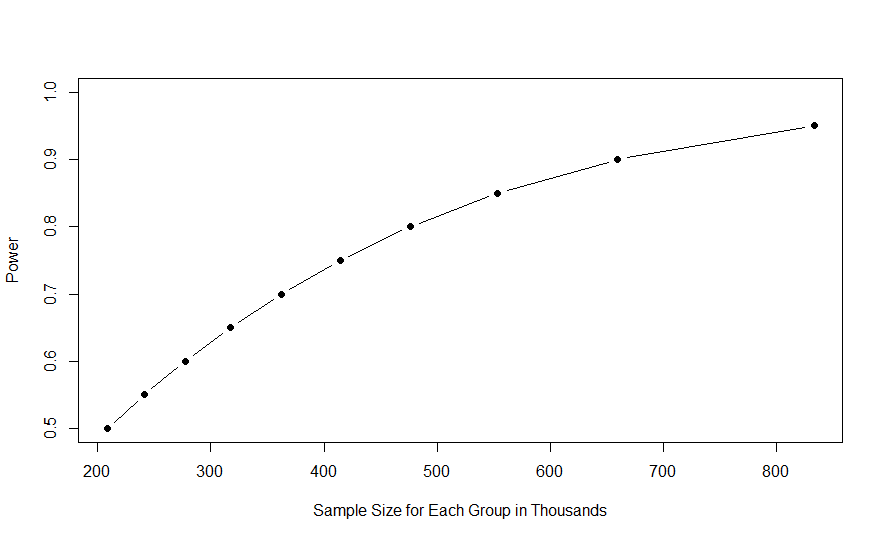
\includegraphics[height=4.7cm, trim=0.0cm 0.3cm 0.0cm -0.8cm width=4.7cm]{Images/Illustrative_Power_Calculation.png}
  \caption{Figure {\color{franklinblue} 3}: Power Analysis Curve for a Two Sample T-Test\footnote{Effect Size: $0.8\vcenter{\hbox{\mbox{\textcent}}}$.  Pooled Standard Deviation: \$1.57. Significance Level: 0.10. Two-sided alternative hypothesis.}}
\end{figure}
\end{frame}

\section{Analyzing Results}

\begin{frame}[t]{A CPG Digital Advertising Campaign}
Suppose a consumer packaged goods (CPG) manufacturer ran an ad campaign announcing a new product line extension for a particular brand.\footnote{While this case study is similar to the one presented in Module 1, there are differences.}  The campaign was solely executed on a particular digital platform.  \\
\vspace{1.5ex}
Suppose the company that owns the digital platform has many \underline{user-level} attributes, such as gender, age, location, \ldots, browsers, operating systems, \ldots, written content created by the user, content provided by the user via camera feature,  content a user viewed or interacted with,  \ldots,  \\
\vspace{1.5ex}
The aforementioned attributes are used to select an \underline{audience}, which is a set of users who may be exposed to an ad of the focal campaign. 
\end{frame}

\begin{frame}[t]{Intent-to-Treat}
A test group user's exposure is a function of the user logging into the platform, the digital platform's targeting algorithms, and the bidding process.  \\
\vspace{1.5ex}
The audience chosen for the campaign summarized must have had a frequent shopper card (FSC) and must have had at least \$75 in monthly total FSC gross value sales for 10 of the 12 months before the campaign commenced.\footnote{Recall the FSC historical purchase requirement is referred to as a \textit{static}. Using a static ensures that a user is using his/her/their FSC cards with some cross-time regularity.}  The FSC requirement permits test and control group users to be linked to sales outcomes such that sales ad effectiveness can be determined.\footnote{In the A/B testing lexicon of the platform, the test group is `A' and the control group is `B'.} 
\end{frame}

\begin{frame}[t]{Ad Campaign Objectives}
The campaign ran for 6 weeks, where in addition to increasing awareness and consideration of the line extension, increasing brand conversion rates, average brand purchase occasions, and average value (i.e., U.S. dollar) sales.  The sales outcome post campaign period was 2 weeks. The design was after-only. \\
\vspace{1.5ex}
 Since the treatment, a brand ad, cannot always be guaranteed to be delivered and the targeting process occurs after a user is assigned to either the test and control group, an intent-to-treat (ITT) testing approach was used to determine the sales effectiveness of the campaign.  Fifty percent of the audience was randomly assigned to the test group and fifty percent to the control group.\footnote{For additional information on the ITT approach, see \cite{gordon2019}. } 
\end{frame}

\begin{frame}[t]{Campaign Exposure Contingency Table}
\small
Elements of the deliverables provided by the platform after the campaign has completed are a set of contingency tables.   \\
\vspace{1.5ex}
\tiny
\begin{table}[ht]
\centering
\begin{tabular}{ll rr |r}
  \toprule
 \multirow{2}*{Age} & \multirow{2}*{Gender} &  \multicolumn{2}{c}{Exposure} & \multicolumn{1}{c}{\multirow{2}*{Total}} \\
 \cmidrule{3-4}
  & &  \multicolumn{1}{c}{No} & \multicolumn{1}{c}{Yes} & \\ 
   \midrule
 18-29      & Unknown/Other                  &   9,678 &   1,136 & 10,814\\ 
             & Male                          &  44,431 &  19,847 & 64,278\\ 
             & Female                        &  72,625 &  24,639 & 97,264\\ 
  30-39      & Unknown/Other                 &  14,532 &   1,809 & 16,341\\ 
             & Male                          &  65,942 &  30,618 & 96,560\\ 
             & Female                        & 107,748 &  38,106 & 145,854\\ 
  40-49      & Unknown/Other                 &  14,821 &   1,939 & 16,760\\ 
             & Male                          &  67,277 &  32,504 & 99,781\\ 
             & Female                        & 108,571 &  40,911 & 149,482\\ 
  50-59      & Unknown/Other                 &   9,362 &   1,195 & 10,557\\ 
             & Male                          &  42,671 &  20,038 & 62,709\\ 
             & Female                        &  68,881 &  24,968 & 93,849\\ 
  60+        & Unknown/Other                 &   45,71 &    545  & 5,116\\ 
             & Male                          &  21,043 &   9,470 & 30,513\\ 
             & Female                        &  34,400 &  11,668 & 46,068\\ 
  Unknown    & Unknown/Other                 &   2,994 &    423  & 3,417\\ 
             & Male                          &  13,607 &   6,568 & 20,175\\ 
             & Female                        &  22,170 &   8,292 & 30,462\\ 
  \midrule 
  \multicolumn{2}{c}{Total}                  & 725,324 &  274,676 & 1,000,000\\
  \bottomrule
\end{tabular}                                
  \caption{Campaign Exposure-Demographic Table}
  \label{tab:adcamp1}%
\end{table}
\end{frame}

\begin{frame}[t]{Campaign Test Variant Contingency Table}
\tiny
\begin{table}[ht]
\centering
\begin{tabular}{ll rr |r}
  \toprule
 \multirow{2}*{Age} & \multirow{2}*{Gender} &  \multicolumn{2}{c}{Test Variant} & \multicolumn{1}{c}{\multirow{2}*{Total}} \\ 
 \cmidrule{3-4}
  & &  \multicolumn{1}{c}{Test} & \multicolumn{1}{c}{Control} & \\ 
   \midrule
  18-29      & Unknown/Other                   &  5,458 &    5,356 & 10,814\\ 
             & Male                            & 32,060 &   32,218 & 64,278\\ 
             & Female                          & 48,853 &   48,411 & 97,264\\ 
  30-39      & Unknown/Other                   &  8,114 &    8,227 & 16,341\\ 
             & Male                            & 48,258 &   48,302 & 96,560\\ 
             & Female                          & 73,008 &   72,846 & 145,854\\ 
  40-49      & Unknown/Other                   &  8,303 &    8,457 & 16,760\\ 
             & Male                            & 49,920 &   49,861 & 99,781\\ 
             & Female                          & 74,799 &   74,683 & 149,482\\ 
  50-59      & Unknown/Other                   &  5,296 &    5,261 & 10,557\\ 
             & Male                            & 31,527 &   31,182 & 62,709\\ 
             & Female                          & 46,903 &   46,946 & 93,849\\ 
  60+        & Unknown/Other                   &  2,602 &    2,514 & 5,116\\ 
             & Male                            & 15,338 &   15,175 & 30,513\\ 
             & Female                          & 22,978 &   23,090 & 46,068\\ 
  Unknown    & Unknown/Other                   &  1,774 &    1,643 & 3,417\\ 
             & Male                            & 10,043 &   10,132 & 20,175\\ 
             & Female                          & 15,248 &   15,214 & 30,462\\
    \midrule 
  \multicolumn{2}{c}{Total}                   & 500,482 &  499,518  & 1,000,000 \\ 
   \bottomrule
\end{tabular}
 \caption{Campaign Test Variant-Demographic Table}
  \label{tab:adcamp2}%
\end{table}
\small
\vspace{-3.0ex}
Table \ref{tab:adcamp2} suggests that the random assignment of a user to a test or control group is working as planned. 
\end{frame}

\begin{frame}[t]{Campaign Test Variant-Exposure Table}
\small
\begin{table}[ht]
\centering
\begin{tabular}{l rr|r}
 \multirow{2}*{Exposure} &  \multicolumn{2}{c}{Test Variant} &  \multicolumn{1}{c}{\multirow{2}*{Total}}\\
 \cmidrule{2-3}
  &  \multicolumn{1}{c}{Test} & \multicolumn{1}{c}{Control} & \\
  \toprule
   \midrule
 No                                  & 225,806 &  499,518 & 725,324\\ 
 Yes                                 & 274,676 &       0  & 274,676\\ 
   \midrule 
  Total                   & 500,482 &  499,518  & 1,000,000 \\ 
   \bottomrule
\end{tabular}
 \caption{Campaign Test Variant-Exposure Table}
  \label{tab:adcamp3}%
\end{table}
\normalsize
\vspace{-2.0ex}
As may be expected, no user in the control group was exposed to a campaign ad. \\
\vspace{1.5ex}
55.3\% of test group users were exposed to campaign ad. \\
\vspace{1.5ex}
In practice, a set of statistical tests would be conducted to determine if the test and control groups were balanced, say by age and gender. \\
\vspace{1.5ex}
\end{frame}

\begin{frame}[t]{Campaign Sales Effectiveness}
\small
Table \ref{tab:adcamp4} contains large sample test results for conversion rate, average purchase occasions, and average value sales. Obviously the campaign was not sales outcome effective.\footnote{If the sample was small and purchase occasions and value sales are normally distributed, and given the unknown variances, one would use a $t$-test in lieu of the large sample test.  A small sample test of proportions could use bootstrap tests (\cite{efron1993} and \cite{shao1996}).} \\
\vspace{1.5ex}
\scriptsize
\begin{table}[ht]
\centering
\begin{tabular}{c l r r}
\multicolumn{1}{c}{Outcome} & \multicolumn{1}{c}{Measure}  & \multicolumn{1}{c}{Test} 
& \multicolumn{1}{c}{Control} \\
\toprule
\multirow{3}*{Conversion Rate}      & Point Estimate & 0.0163 & 0.0160 \\
                                    & Alternative Hypothesis & \multicolumn{2}{c}{Two-Sided} \\
                                    & $p$-value & \multicolumn{2}{c}{0.3639} \\
 \cmidrule{2-4}
 Average                            & Point Estimate & 0.0171 & 0.0168 \\
 Purchase                           & Alternative Hypothesis & \multicolumn{2}{c}{Two-Sided} \\
 Occasions                          & $p$-value & \multicolumn{2}{c}{0.2878}  \\
                                 
 \cmidrule{2-4}
 Average                            & Point Estimate & \$0.1922  & \$0.1885 \\
 Value                             & Alternative Hypothesis & \multicolumn{2}{c}{Two-Sided} \\
 Sales                              & $p$-value & \multicolumn{2}{c}{0.2741}  \\
 \bottomrule
\end{tabular}
 \caption{Campaign Sales Effectiveness Using Test/Control Groups}
  \label{tab:adcamp4}%
\end{table}
\end{frame}

\begin{frame}[t]{Be Wary of Exposed/Unexposed Group Test Results}
\small
If we \underline{only} knew users who were exposed and not exposed, that is we do not know which test variant a user was assigned, we would have an observational data study.  Thus one may wish to conduct statistical inference with exposed and unexposed groups.\footnote{Note it is not appropriate to conduct such an exercise, either from a statistical or causal inference point of view, without proper statistical adjustments.  Potential approaches are mentioned later in this section. }
\scriptsize
\begin{table}[ht]
\centering
\begin{tabular}{c l r r}
\multicolumn{1}{c}{Outcome} & \multicolumn{1}{c}{Measure}  & \multicolumn{1}{c}{Exposed} 
& \multicolumn{1}{c}{Unexposed} \\
\toprule
\multirow{3}*{Conversion Rate}      & Point Estimate & 0.0170 & 0.0158 \\
                                    & Alternative Hypothesis & \multicolumn{2}{c}{Two-Sided} \\
                                    & $p$-value & \multicolumn{2}{c}{$<0.0001$}  \\
 \cmidrule{2-4}
 Average                            & Point Estimate & 0.0179 & 0.0168 \\
 Purchase                           & Alternative Hypothesis & \multicolumn{2}{c}{Two-Sided} \\
 Occasions                          & $p$-value & \multicolumn{2}{c}{$<0.0001$}  \\
                                 
 \cmidrule{2-4}
 Average                            & Point Estimate &  \$0.2038 &  \$0.1854 \\
 Value                             & Alternative Hypothesis & \multicolumn{2}{c}{Two-Sided} \\
 Sales                              & $p$-value & \multicolumn{2}{c}{$<0.0001$}  \\
 \bottomrule
\end{tabular}
 \caption{Campaign Sales Effectiveness Using Exposure Groups}
  \label{tab:adcamp5}%
\end{table}
\small
\vspace{-3.0ex}
\end{frame}

\begin{frame}[t]{Revisiting Causal Inference}
Notice that the exposed outcome estimates of Table \ref{tab:adcamp5} are larger than the control outcome estimates of Table \ref{tab:adcamp4}. \\
\vspace{1.5ex}
Two broadly divided causal inference approach types: 
\begin{enumerate}
\item Statistical adjustment to control confounding and arrive at a causal estimate.  
\begin{itemize}
\item These approaches rely on the assumption that there is no remaining unmeasured confounding and no measurement error after the application of the methods. 
\item Effective statistical adjustment for confounding requires knowing what to measure, and measuring it accurately.
\end{itemize}
\item Design-based methods such as randomized control trials, and its digital space A/B testing implementation.\footnote{The methods do not rely on the supposition that there is no remaining unmeasured confounding and no measurement error. } 
\end{enumerate}
\end{frame}

\begin{frame}[t]{Observational Data Study Causal Inference Methods}
Approaches that rely on statistical adjustment are likely to have similar, or at least related, sources of bias. Design-based approaches are more likely to have different sources of bias. \\
\vspace{1.5ex}
Observational data study methods used in an effort to realize accurate and precise causal inference include, but are not limited to: \\
\vspace{1.5ex}
\begin{enumerate}
\item Matching Methods
\begin{itemize}
\item Exact Matching
\item Stratification
\item Nearest Neighbor Covariate Matching
\item Propensity Scores
\end{itemize}
\end{enumerate}
\end{frame}

\begin{frame}[t]{Instrumental Variables, Matching Methods \ldots}
\begin{enumerate}
  \setcounter{enumi}{1}
\item Instrumental Variables
\item Doubly Robust Estimators
\begin{itemize}
  \item Target Maximum Likelihood
  \item Doubly/Debiased Machine Learning
\end{itemize}
\item Difference-in-Differences
\item Regression Discontinuity
\item Synthetic Control Method
\end{enumerate}
\cite{taddy2023} contains introductions to several of the methods mentioned above. \cite{hernan2020} is a more rigorous treatment of several of the approaches. 

\end{frame}

\begin{frame}[t]{Experimental Design Testing Approaches}
To conduct statistical inference for A/B tests, one typically uses large sample tests or t-tests.  These tests yield \empr{frequent statistics}. Table \ref{tab:adcamp4} tests are large sample frequentist tests. \\
\vspace{1.5ex}
An alternative to the frequentist approach to testing is \empr{Bayesian statistical inference}. It is an approach to data analysis and parameter estimation based on Bayes' theorem.\footnote{The Appendix contains a brief review of Bayes' theorem.} \\
\vspace{1.5ex}
Unique for Bayesian statistics is that all observed and unobserved parameters in a statistical model are given a joint probability distribution. \\
\vspace{1.5ex}
\end{frame}

\begin{frame}[t]{Prior, Likelihood and Posterior Distribution}
\begin{enumerate}
\item \empr{Prior distribution}:  It is the beliefs held by researchers about the parameters in a statistical model before seeing the data, expressed as probability distributions.
\item \empr{Likelihood function}: The conditional probability distribution of the observed data given the parameters, defined up to a constant. This is called a likelihood because for a given pair of data and parameters it registers how `likely' is the data.
\item \empr{Posterior distribution}: A way to summarize one's updated knowledge, balancing prior knowledge with observed data, and is used to conduct inferences. More precisely, the likelihood is combined with the prior distribution to form the posterior distribution.
\end{enumerate} 
\end{frame}

\begin{frame}[t]{Posterior Distribution Specification}
\small
The posterior distribution results from applying Bayes' rule.  Let $D$ represent the data and $\theta$ the parameters of interest (e.g., means, proportions, regression coefficients \ldots). An application of Bayes' Rule yields. \\
\vspace{0.0ex}
\begin{equation}
P(\theta|D) = \frac{P(D|\theta) P(\theta)}{P(D)}, \;\;\; \text{where:} 
\end{equation} 
\vspace{-1.5ex}
\begin{itemize}
 \item $P(\theta)$ is the prior distribution. This is the strength in our belief of $\theta$ without considering the evidence.
\item  $P(D|\theta)$ is the likelihood function. This is the probability of observing the data as generated by a model with parameter $\theta$.
\item $P(D)$ is the evidence. This is the probability of the data as determined by summing (or integrating) across all possible values of $\theta$, weighted by how strongly we believe in the particular values of $\theta$. 
\item $P(\theta|D)$ is the posterior distribution. This is the refined belief of $\theta$  once the evidence   has been taken into account.
\end{itemize}
\end{frame}

\begin{frame}[t]{Bayesian Inference is Becoming More Popular}
For every frequentist approach to a particular statistical problem, there is usually at least one Bayesian approach. For example, there are many Bayesian one-sample and two-sample t-test variants.\footnote{Examples include those of \cite{gonen2005}, \cite{wang2016}, \cite{abdelrazeq2020}, \cite{gronau2020}, and \cite{alLabadi2022}.} \\
\vspace{1.5ex}
Bayesian inference can be computationally demanding.  As computation has become more efficient and cost-effective, Bayesian inference popularity and use has experienced increased industry use.
\end{frame}

\begin{frame}[t]{Analysis of Variance}
Recall that an A/B test is only one type of experiment.  Specifically, it is  \textit{a field experiment in the digital world}. A/B tests have 1 factor with 2 treatments. \\
\vspace{1.5ex}
For tests with multiple factors and hence potential interactions, we may wish to compare many pairs of treatments at the same time.  One method to conduct such inference is via Analysis of Variance (ANOVA). ANOVA allows for simultaneous comparisons of more than two factors.\footnote{As an example consider the previously discussed different women's category landing page where ``above-the-fold'' shows one of two items, where each item could be one of three colors.  For these two factors, there are $2 \times 3 = 6$  interactions.}\\
\vspace{0.0ex}
\small
\begin{itemize}
\item While the main result of an ANOVA is again the $p$-value, this time the $p$-value is associated with an F-statistic.  
\item The F-statistic can handle more factors than the one factor standard normal statistics (i.e., ``z statistics'') and t-statistics. 
\end{itemize}
\end{frame}

\begin{frame}[t]{A Retailer Experimental Design}
%https://stat.ethz.ch/~meier/teaching/anova/random-and-mixed-effects-models.html
%https://www.scribbr.com/statistics/anova-in-r/
A mall-based retailer with stores nationwide is considering changing its front-facing windows and store-layout, or ``floorset''.  Before making such changes, the company wants to ensure that the change will have a positive effect on store revenue.  In particular, the proposed changes would ideally result in larger gross value sales per store selling foot. Of the more than 1,000 stores, 80 stores were randomly selected to participate in the test. \\
\vspace{1.5ex}
The company designed the following test: 
\begin{itemize}
\item Total number of Stores:  80
\item Factor 1:  Window ($W$)
\small
  \begin{itemize}
  \item Treatment $W_1$:  Window display from last year.  Referred to as the \textit{champion window}.
  \item Treatment $W_2$:  Proposed new window display.  Referred to as the \textit{challenger window}.
\end{itemize}
\end{itemize}
\end{frame}

\begin{frame}[t]{A Retailer Experimental Design Continued}
\begin{itemize}
 \item []
 \small
 \begin{itemize}
  \item   50\% of the 80 stores were randomly selected to be assigned $W_2$.  The other 50\% of stores were assigned $W_1$.
 \end{itemize}
 \normalsize
 \item Factor 2:  Floorset ($FS$)
 \small
  \begin{itemize}
  \item Treatment $FS_1$:  Floorset from last year.  Referred to as the \textit{champion floorset}.
  \item Treatment $FS_2$:  Proposed new floorset.  Referred to as the \textit{challenger floorset}.
  \item 
  50\% of the 80 stores were randomly assigned $FS_2$.  The other 50\% of stores were assigned $FS_1$. 
\end{itemize}
\normalsize
\item This design has 2 factors, each with 2 levels, and thus there is the possibility of an interaction effect.
\item The test window is 4 weeks. 
\end{itemize}
\end{frame}

\begin{frame}[t]{Visualizing the Data}
We should take a look at the data before conducting statistical inference via an ANOVA. \\
\vspace{1.5ex}
\begin{figure}[htbp]
  \captionsetup{justification=centering}
  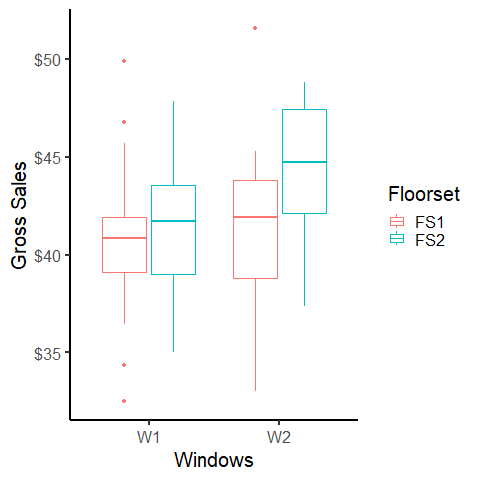
\includegraphics[height=5.4cm, trim=0.0cm 0.0cm 0.0cm 0.0cm width=5.4cm]{Images/Summary_stats.png}
  \caption{Figure {\color{franklinblue} 4}: Boxplot of Window and Floorset Treatment Gross Sales per Selling Square Foot Across Stores}
\end{figure}
\end{frame}

\begin{comment}
\begin{table}[t]{Visualizing the Data Continued}
The main purpose of a plot  this is to help us understand what the treatments are doing. We want to quickly assess things like: 
\begin{itemize}
\item How big are the main effects? 
\item What direction do they work in? 
\item Is there likely to be an interaction?
\end{itemize}
\end{frame}
\end{comment}

\begin{frame}[t]{ANOVA Specification}
For $i$ indexing a store, $j=\{W_1,W_2\}$, and $k=\{FS_1,FS_2\}$, the two-way ANOVA specification for this test is: \\
\vspace{-1.0ex}
\begin{equation}
Y_{ijk} = \mu + \alpha_j + \beta_k + (\alpha\beta)_{jk} + \epsilon_{ijk},
\end{equation}
where $\epsilon_{ijk} \sim \text{N}(0,\sigma^2)$ are independent and $\sum_{\forall j} \alpha_j = \sum_{\forall k} \beta_k = \sum_{\forall j, \forall k}(\alpha_j \beta_k) = 0$. \\
\vspace{1.5ex}
Using the estimated coefficients of the model, we may test treatment \empr{contrasts}. \\
\vspace{1.5ex}
A contrast is essentially a difference in regression coefficients.
\end{frame}

\begin{frame}[t]{Interpreting the ANOVA Table}
The table below is the ANOVA table for the retailer's test design. \\
%trim={<left> <lower> <right> <upper>}
%\vspace{-2.5ex}
%\begin{figure}[htbp]
%  \captionsetup{justification=centering}
%  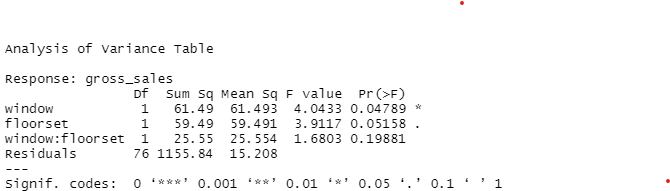
\includegraphics[height=3.2cm, trim=0.0cm 0.0cm 0.0cm 0.8cm width=3.2cm]{Images/ANOVA_Output.png}
%  \caption{Figure {\color{franklinblue} xx}: ANOVA Table for Retailer Window and Floorset Test}
%\end{figure}
\small
\verbatiminput{Images/ANOVA_Statistics.txt}
\normalfont
%\vspace{-2.0ex}
\begin{enumerate}
  \item The upper part of the table tells us we are looking at an ANOVA table where the outcome (i.e., response) was \texttt{gross\_sales}, which is truly gross value sales.
\end{enumerate}
\end{frame}

\begin{frame}[t]{Interpreting the ANOVA Table Continued}
\begin{enumerate}
  \setcounter{enumi}{1}
  \item The 3 lines that begin with \texttt{window} value are for testing the following null hypotheses:
  \begin{itemize}
    \item $H_{0,W}\text{:}$  Gross sales per selling square foot of the challenger window is equal to that of the champion window. 
    \item $H_{0,FS}\text{:}$  Gross sales per selling square foot of the challenger floorset is equal to that of the champion floorset. 
    \item  $H_{0,W \times FS}\text{:}$ There is no gross sales per selling square foot interaction effect for the challenger window and challenge floorset.
  \end{itemize}
 \item The alternative for each null hypothesis is two-sided.
\end{enumerate}
\end{frame}

\begin{frame}[t]{Interpreting the ANOVA Table Continued}
\begin{enumerate}
  \setcounter{enumi}{3}
 \item The \texttt{F value} is the test statistic for each variable (i.e., factor or interaction of factors). These provide a measure of how large and consistent the effects associated with each variable are. Each \texttt{F value} has a pair of degrees of freedom associated with it: one belonging to the variable itself, the other due to the error (residual). Together, the \texttt{F value} and its degrees of freedom determines the $p$-value, which is \texttt{Pr(>F)} in the table.
 \item The $p$-value gives the probability that the differences between the set of means for each variable in the model, or a more extreme difference, could have arisen through sampling variation under the null hypothesis of no difference.
 \item The ANOVA table tells us nothing about the direction of the effects.  Via the least squares fit of the model, we have the following estimates:  $\hat{\mu} = 40.80$, $\hat{\alpha}_{W_2} = 0.62$, $\hat{\beta}_{FS_2} = 0.59$ and the interaction coefficient for $FS_2$ and $W_2$ is $ \hat{\gamma}_{W_2,FS_2} =  2.26$ .
\end{enumerate} 
\end{frame}

\begin{frame}[t]{Average Gross Value Sales Effectiveness}
\begin{figure}[htbp]
  \captionsetup{justification=centering}
  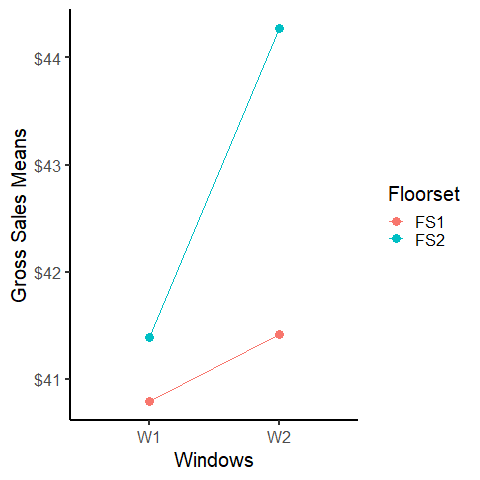
\includegraphics[height=5.2cm, trim=0.0cm 0.0cm 0.0cm 0.0cm width=5.2cm]{Images/ANOVA_RESULTS.png}
  \caption{Figure {\color{franklinblue} 5}: Average Gross Value Sales Per Selling Square Foot \\ For Each Factor's Treatment}
\end{figure}
\vspace{-2.0ex}
\small
Based on these results, do you think the business should implement the challenger floorset, the  challenger window, both, or none?  What are the reasons for your answer?
\end{frame}

\section{Appendix}

\begin{frame}[t]{The General Multiplication Rule for Probabilities}
For two events $A$ and $B$, the \empr{General Multiplication Rule for Probabilities} is $P(A \cap B) = P(A)P(B|A)$. \\
\vspace{1.5ex}
Two events are \empr{independent} if the occurrence of one does not affect the probability that the other event occurs. If two events are not independent, we say they are \empr{dependent}. \\
\vspace{1.5ex}
The \empr{Multiplication Rule for Independent Events} says if $A$ and $B$ are independent events, then 
\begin{equation}
P(A \cap B) = P(A) P(B).
\end{equation}
This rule can be extended to the case where there are more than two independent events. If $A, B, C, \ldots $ are independent events, then
\begin{equation}
P(A \cap B \cap C \cap \ldots) = P(A) P(B) P(C)\ldots.
\end{equation}
\end{frame}

\begin{frame}[t]{Adjusting Probability Statements}
\empr{Bayes' theorem} provides a way of revising conditional probabilities by using available information. It also provides a procedure for determining how probability statements should be adjusted, given additional information. \\
\vspace{1.5ex}
Reverend Thomas Bayes (1702–1761) developed Bayes’ theorem, originally published
in 1763 after his death and again in 1958. Because games of chance — and, hence, probability — were considered to be works of the devil, the results were not widely publicized. \\
\vspace{1.5ex}
Since World War II a major area of statistics and a major area of management decision theory have developed based on the original works of Thomas Bayes.
\end{frame}

\begin{frame}[t]{Reverend Thomas Bayes}
\begin{textblock*}{5cm}(1cm,2.50cm)
\begin{figure}[htbp]
  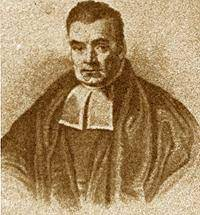
\includegraphics[height=1.3in]{Images/bayes.jpg}
  \caption{Reverend Thomas Bayes}
\end{figure}
\end{textblock*}
\begin{textblock*}{5cm}(6cm,2.50cm)
\begin{figure}[htbp]
  
\includegraphics[height=1.3in]{Images/Bayes-DivineBenevolence.jpg}
  \caption{\textit{Divine Benevolence}}
\end{figure}
\end{textblock*}
\small
 Bayes' first publication was a theological work, \textit{Divine Benevolence}, where he was trying to address the motivating source of God's actions.\footnote{Since no author appears on the title page of \textit{Divine Benevolence}, or anywhere else, it is sometimes considered to be of doubtful authorship. For example, the \href{https://www.loc.gov/coll/nucmc/}{\textit{National Union Catalog}} ascribes authorship to Joshua Bayes. However, Thomas Bayes was probably the author of this work. Richard Price, a friend of Bayes,  refers to the book in his own work \textit{A Review of the Principal Questions in Morals}, and says that it was written by Thomas Bayes.} 
\end{frame}

\begin{frame}[t]{Bayes Theorem}
 Let $A$ and $B$ be two events with respective probabilities $P(A)$ and $P(B)$.  The General Multiplication Rule for Probabilities gives
\begin{equation} \label{eq:bayes1} 
P(A \cap B) = P(B|A)P(A), 
\end{equation}
and also
\begin{equation} \label{eq:bayes2} 
P(A \cap B) = P(A|B)P(B). 
\end{equation}
\\
\vspace{0.5ex}
Since the left-hand sides of Equations (\ref{eq:bayes1}) and (\ref{eq:bayes2}) are the same, so must the fight hand sides, so that $P(B|A)P(A)  = P(A|B)P(B)$. Dividing through this equation by $P(A)$, assuming it is not zero, gives Bayes theorem:  For any two events $A$ and $B$ where $P(A) >0$,
\vspace{0.5ex}
\begin{equation} \label{eq:bayes3} 
P(B|A) = \frac{P(A|B)P(B)}{P(A)}. 
\end{equation}
\end{frame}

\begin{frame}[t]{Subjective Probability Interpretation}
The most interesting interpretation of Bayes' theorem is in terms of \underline{subjective} probabilities. \\
\vspace{0.5ex}
\small
\begin{itemize}
  \item Suppose an individual is interested in the event $B$ and forms a subjective view of the probability that $B$ will occur;  in this context $P(B)$ is called a \empr{prior} probability. 
  \item If the individual acquires an additional piece of information -- namely, that event $A$ has occurred -- this may cause a modification of the initial judgement as to the \empr{likelihood} of the occurrence of $B$. 
  \item Since $A$ is known to have happened, the relevant probability for $B$ is now $P(B|A)$, which is referred to as the \empr{posterior} probability.
  \item Thus Bayes' theorem can be thought as a mechanism to update a prior probability to a posterior probability when the additional information that event $A$ has occurred becomes available. The mechanism is by a multiplication of $P(B)$;  specifically, by $P(A|B)/P(B)$. \\
\end{itemize}
\end{frame}

\begin{frame}[t]{Extending Bayes Theorem}
Bayes theorem is often expressed in a different but equivalent form.  Let $E_1, E_2, \ldots, E_K$ be $K$ mutually exclusive and collectively exhaustive events, and let $A$ be some other event.  \\
\vspace{1.5ex}
For some $i$, we want to find $P(E_i|A)$.  This can be obtained directly by Bayes' theorem by setting $B$ in Equation (\ref{eq:bayes3}) equal to $E$.  \\
\vspace{1.5ex}
However, the denominator on the right-hand side of that equation can be expressed in terms of conditional probabilities for $A$ given the $E_j$ and probabilities of each $E_j$.  Thus it follows that 
\begin{equation} \label{eq:bayes4}
P(A) = \sum_{k=1}^{K} P(E_k \cap A).
\end{equation}
\end{frame}

\begin{frame}[t]{An Alternative Statement of Bayes Theorem}
Furthermore using the General Multiplication Rule for Probabilities, $P(E_j \cap A) = P(A|E_j)P(E_j)$, $j \in \{1,2,\ldots,K\}$, we have \\
\vspace{-0.5ex}
\begin{equation} \label{eq:bayes5}
P(A) = \sum_{k=1}^{K} P(A|E_k)P(E_k).
\end{equation}
Finally, the restatement of Bayes' theorem is obtained by substituting $E_i$ for $B$ and the right-hand side of Equation (\ref{eq:bayes5}) for $P(A)$ in Equation (\ref{eq:bayes3}).  Thus assuming at least one $P(E_j)>0$, $j \in \{1,2,\ldots, K\}$, the \underline{alternative statement of Bayes' theorem} is \\
\vspace{-0.5ex}
\begin{equation} \label{eq:bayes6}
P(E_i |A ) = \frac{P(A|E_i)P(E_i)}{\sum_{k=1}^{K} P(A|E_k)P(E_k)}.
\end{equation}  
\end{frame}

\begin{comment}

\begin{frame}[t]{Are Delinquent Girls Likely to be the Youngest?}
A research study investigated the possible relationship between delinquency and birth order of high school girls.\footnote{This vein of research has been on-going for more than a hundred years.  One of the earliest studies is, Breckinridge, S. P. and Abott, E. (1912). \textit{The Delinquent Child and the Home}, Russell Sage. New York, NY.  One of the first studies focusing on the delinquency of girls and birth order is, Cowie, J., Cowie, V., and Slater, E. (1968). \textit{Delinquency in Girls}.  Heinemann Educational. London, England.}  \\
\vspace{1.5ex}
Delinquency ($D$) was somewhat arbitrarily defined according to answers on a questionnaire.  Of the girls in the study, 40\% were the eldest ($E$), 30\% middle ($M$), 20\% youngest ($Y$), and 10\% were the only child in the family ($O$). The delinquency percentage \underline{given} the child is the eldest is  5\%, the child is middle 10\%, the child is youngest 15\%, and child is an only child is 20\%.  What is the probability that a delinquent girl is the youngest in their family? \\
\end{frame}

\begin{frame}[t]{Delinquent Girls Continued}
\underline{Solution}: \\
\vspace{1.5ex}
Since the age classification of girls is mutually exclusive and collectively exhaustive, we may use Bayes theorem to address the question. \\
\vspace{-0.5ex}
\footnotesize
\begin{align} \nonumber
\begin{split}
P(Y | D) & = \frac{P(D|Y)P(Y)}{P(D|E)P(E) +  P(D|M)P(M) + P(D|Y)P(Y) + P(D|O)P(O)} \\
&  \\
& = \frac{0.15\times0.20}{(0.05\times0.40) + (0.10\times0.30) + (0.15\times0.20) + (0.20\times0.10)}\\
& \\
& = \frac{0.03}{0.10} \\
& \\
& = 0.30
\end{split}
\end{align}  
\end{frame}

\end{comment}

\begin{frame}[t]{Spam Emails}
\href{https://www.spamlaws.com/spam-stats.html}{Spamlaws} estimates that 45\% of emails are spam emails. Many email service providers deploy software to filter spam emails before they reach an inbox. A particular software solution claims that it can detect 99\% of spam emails, and the probability for a false positive, a non-spam email detected by the software as spam, is 5\%. \\
\vspace{1.5ex}
If an email is detected as spam, what is the probability that it is truly a non-spam email? \\
\end{frame}

\begin{frame}[t]{Spam Emails Continued}
\small
\underline{Solution}: \\
\vspace{1.5ex}
First, the following events are defined. \\
\vspace{-1.5ex}
\begin{align} \nonumber
\begin{split}
A & = \text{event that an email is detected as spam,} \\
B & = \text{event that an email is spam,} \\
B^c & = \text{event that an email is not spam.}
\end{split}
\end{align}  
\\
\vspace{0.5ex}
From above we know, $P(B) = 0.45$, $P(B^c) = 0.55$, $P(A|B) = 0.99$, and $P(A|B^c) = 0.05.$   By Bayes' theorem, \\
\vspace{0.0ex}
\begin{align} \nonumber
\begin{split}
P(B^c|A) & =  \frac{P(A|B^c)P(B^c)}{P(A|B)P(B)+P(A|B^c)P(B^c)}, \\
 & = \frac{0.05\times0.55}{ (0.99\times 0.45) +(0.05\times0.55)},  \\
& = \frac{0.028}{0.028 + 0.446}, \\
& = 0.058.
\end{split}
\end{align}
\end{frame}

\section{References}

\begin{frame}[t,allowframebreaks]
%https://latex-beamer.com/faq/long-bibliographies-beamer/
%https://github.com/jgm/pandoc/issues/2442
\widowpenalties 1 10000
\small
\bibliography{../../Bibliography/list2}
\bibliographystyle{apalike}
\end{frame}

\end{document}